\section{Design \& Implementation}
This section contains information about the design and implementation of the robot in this project.

\subsection{Overall Design}
The overall system design can be seen in figure \ref{fig:OSD}. The connection between the Computer and the Bluetooth shield is wireless. The connection between the Bluetooth shield and the Arduino Uno is serial. The connection between the Arduino Uno and LIDAR Sensor is serial and lastly the connection between the Arduino Robot and the Arduino Uno is i2c.
\begin{figure}[H]
\centering
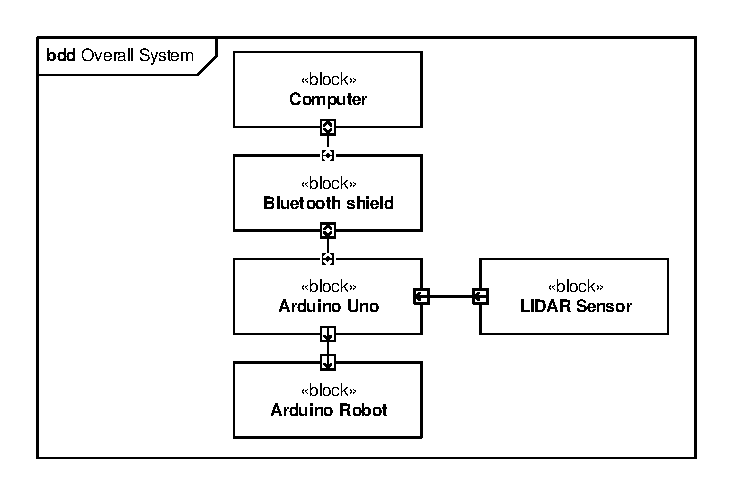
\includegraphics[width=0.7\textwidth]{billeder/OverallSystemDesign}
\caption{Overall System Design}
\label{fig:OSD}
\end{figure}

\subsection{Computer}
The computer has the responsibility to take the measurement data from the Bluetooth shield and process it. The processing is done in Matlab. 

\subsection{Bluetooth shield}
The Bluetooth shield is an "ITEAD Wireless Bluetooth Shield Module Starter Kit For Arduino"\cite{BTshield}\cite{BTshield2}. The responsibility of the Bluetooth shield is to transfer data from the Arduino Uno to the Computer. The shield uses a HC-05 Serial Bluetooth module. Connecting to the shield is done by finding "H-C-2010-06-01" on the Computer and using the password: "1234". The settings for the serial bus is:
\begin{itemize}
\item Default baud rate: 9600
\item Data bits: 8
\item Stop bit: 1
\item No parity
\end{itemize}

\subsection{Arduino Uno}
Arduino Uno\cite{ArduinoUno}.
the Arduino Uno handles communication with the LIDAR Sensor and the Bluetooth shield.
\begin{figure}[H]
\centering
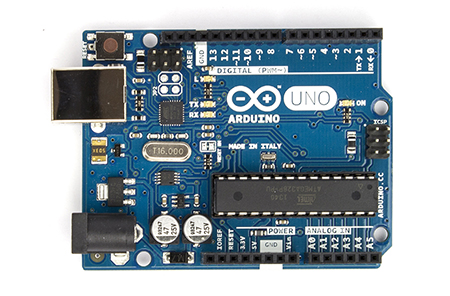
\includegraphics[scale=0.5]{billeder/ArduinoUno}
\caption{Arduino Uno}
\label{fig:ArduinoUno}
\end{figure}

\subsection{LIDAR Sensor}
A LIDAR measurement consists of 90 packets with four range measurements in each. The packet length is 22 bytes and is organised as follows\cite{LIDAR}:
\begin{verbatim}
<start> <index> <speed_L> <speed_H> [Data 0] [Data 1] [Data 2] [Data 3]
 <checksum_L> <checksum_H>
\end{verbatim}
The $start$ code is 0xFA, $index$ goes from 0xA0 to 0xF9, $speed$ is the fixed point speed in RPM and $Data$ $N$ is the Nth reading. Each reading is four bytes in length and contains information about distance, signal strength and two flags. The data is comprised as follows:
\begin{verbatim}
<distance 7:0>  <"invalid data" flag> <"strength warning" flag> 
<distance 13:8> <signal strength 7:0> <signal strength 15:8>
\end{verbatim}
The LIDAR, also called Neato LIDAR can be seen in figure \ref{fig:NeatoLidar}.
\begin{figure}[H]
\centering
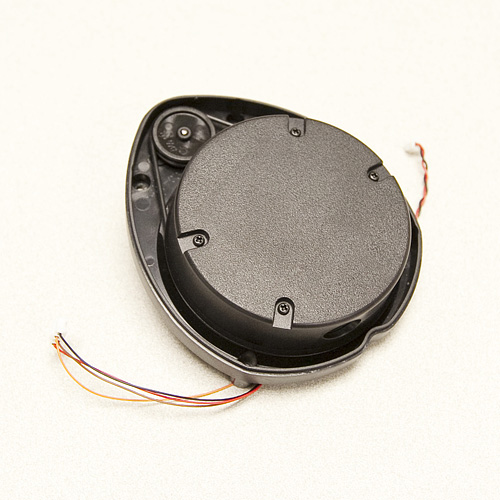
\includegraphics[scale=1]{billeder/NeatoLidar}
\caption{Neato LIDAR Sensor}
\label{fig:NeatoLidar}
\end{figure}
The LIDAR has four connects to the sensor part and two to the motor part. The motor connects are 3.3 Volt based with red being power and black being ground. The pinout for the sensor part is seen in table \ref{tab:lidars}.
\begin{table}[H]
\centering
\begin{tabular}{|l|l|}
\hline
Red & 3.3V \\ \hline
Brown & LDS\_RX \\ \hline
Orange & LDS\_TX \\ \hline
Black & GND \\ \hline
\end{tabular}
\caption{LIDAR Sensor Pinout}
\label{tab:lidars}
\end{table}

\subsection{Arduino Robot}
The robot platform used in this project is a Arduino robot\cite{ArduinoRobot}. The Arduino robot platform handles all movement commands.

 
%------------------------------------------------